\exercisetitle{
Para  el  circuito  mostrado,  encontrar  la  potencia  transmitida  a  la  carga  y  la  potencia  disipada  en  el
generador para una impedancia de carga $Z_L= 30 +j40\Omega$.  ¿Qué valor de la impedancia de carga permitirá una entrega maxima de potencia a la carga?  ¿Cuál es esta potencia?

}
\subsection{$Z_L = 30 + 40 \Omega$}
Procederemos de la siguiente manera:
\begin{enumerate}
  \item Calcularemos la impedancia normalizada de la carga
  \item Situaremos esta impedancia en la carta de smith, obteniendo $\Gamma_L$
  \item Moveremos la línea $0.7\lambda$ hacia el generador para obtener $z_{in}$
  \item Denormalizaremos $z_{in}$ y obtenedremos la potencia entregada a la línea.
\end{enumerate}

\begin{figure}[h]
  \centering
  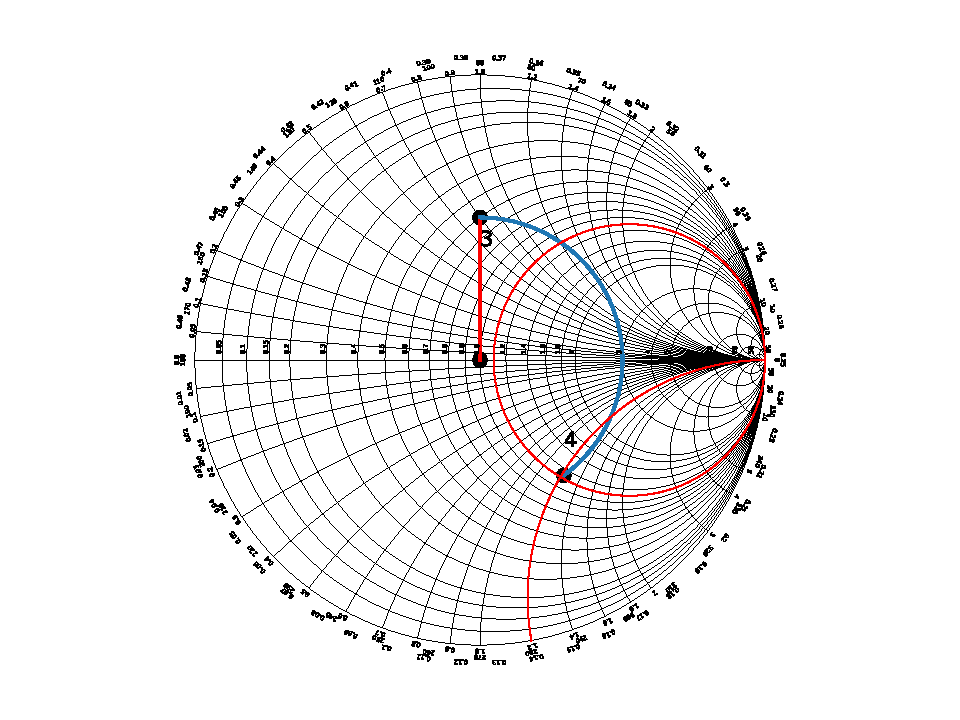
\includegraphics[scale = 0.85]{ej6/images/out1.pdf}
  \caption{Pasos 3 y 4}
  \label{ej2smith}
\end{figure}

En este caso $z_in = \frac{3}{5} + j\frac{4}{5}$, obteniendo, como se puede ver en la figura 2:
\[ \Gamma_L = 0.5e^{j1.57} \]
Tras mover la línea $0.7\lambda$ obtenemos $z_{in} = 1.1 + 1.2j$, que denormalizado queda como:
\[Z_{in} = 55 + 60j\]
 Con lo que podremos calcular la potencia de entrada a la línea con la siguiente expresión:
\begin{align*}
  P_{in} &= \frac{1}{2}|V_S|^2 \frac{R_{in}}{(R_S + R_{in} )^2 + (X_S + X_{in})^2}
  P_{in} &= \frac{1}{2}100  \frac{55}{(20+55)^2 + (30+60)^2}
  P_{in} &= 0.2 W
\end{align*}

Por lo tanto se entregarán 0.2W a la carga, ya que al no tener la línea perdidas, toda este energía se entregará a la carga.

\subsection{¿Qué valor de la impedancia de carga permitirá una entrega maxima de potencia a la carga?}
El valor que hará que esta potencia entregada a la carga sea máxima será el que haga que la impedancia de entrada a la línea sea: $Z_{in} = R_S - X_S$, por que empezaremos normalizando este valor con la impedancia del generador: $z_{in} = 0.4 + 0.6j$. Situaremos este valor en la carta de smith, y retrocederemos hasta la carga $0.7\lambda$, y la impedancia obtenida será la que máximize la potencia entregada  la carga.

\begin{figure}[h]
  \centering
  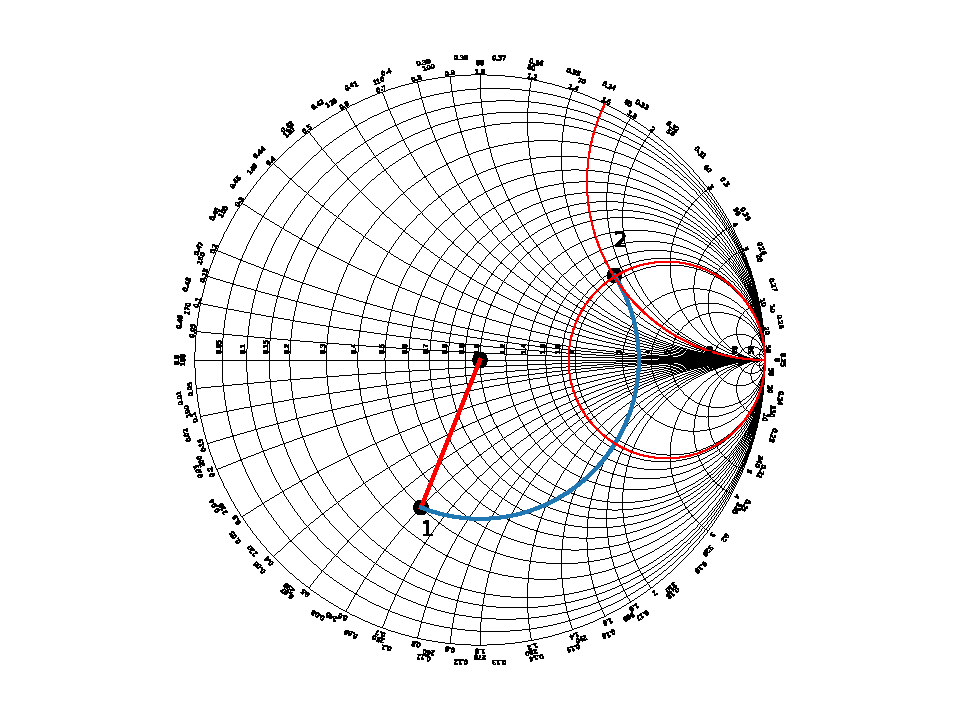
\includegraphics{ej6/images/out2.pdf}
  \caption{Avanzando $0.7\lambda$ hacia la carga}
  \label{ej2smith}
\end{figure}

Donde podemos ver que la impedancia normalizada $z_l = 1.9 +1.6j$, que denormalizada es $Z_L = 95 + 80j \Omega$

\subsection{¿Cuál es esta potencia?}
Podemos usar la expresión de la potencia entregada a la carga cuando la línea esta completamente adaptada a la línea:
\[P_{in} = \frac{|V_s|^2}{8R_s} = 0.625W\]
